\chapter{Multivariate component-wise boosting on survival data}
\label{ch:FHTboost}
In this chapter, we propose a component-wise boosting algorithm for fitting the inverse gaussian first hitting time model to survival data.

\section{FHTBoost}
The first-hitting-time model with Wiener processes, as shown, leads to inverse Gaussian lifetimes. As in the usual
regression scheme (see subsection \ref{subsec:IG-reg}) for this setup, we we have $K=2$ distribution parameters,
\begin{equation}
    \btheta_i=(\theta_1,\theta_2)^T=(y_0,\mu)^T.
\end{equation}
We choose link functions
\begin{equation}
    g_1(x)=\log(x)
\end{equation}
and
\begin{equation}
    g_2(x)=\id(x)=x,
\end{equation}
for parameters $y_0$ and $\mu$, respectively.

We wish to model the effect of covariates on these parameters. In particular, we will let $y_0$ be modeled by a high-dimensional matrix $X$,
in practice typically gene expression data, and we will let $\mu$ be modeled by a low-dimensional matrix $Z$, typically clinical data.
We let a vector of covariate information from one individual $i,i=1,2,\ldots,n$ be labeled $\x_i$ and $\z_i$, where these are
gene data and clinical data, respectively.
These matrices are defined as
\begin{equation}
    X=(\x_1,\x_2,\ldots,\x_{p_1}),
\end{equation}
and
\begin{equation}
    Z=(\z_1,\z_2,\ldots,\z_{p_2}),
\end{equation}
where the number of dimensions $p_1$ of $X$ is high (in particular, $p_1$ is much larger than $n$, $p_1 >> n$),
and the number of dimensions $p_2$ of $Z$ is relatively small, and in particular, $p_2 < n$.

We apply the GAMLSSBoost algorithm shown previously (see section \ref{sec:gamlssboost}) to this setup. The loss function of interest is
the negative log likelihood of the censored inverse Gaussian distribution, derived in the Appendix, i.e.,
\begin{equation*}
    \rho(y,\btheta)=-l((t,d), (y_0,\mu)).
\end{equation*}
(See Appendix for the full expression!)
We wish to build up an additive predictor $\boldeta$, consisting of components $\eta_1$ and $\eta_2$. As in the GAMLSS setting, these are given by
\begin{equation}
    \eta_1\coloneqq \exp(y_0)=\beta_{1,0}+\sum_{j=1}^{p_1}f_{1,j}(x_{1,j}),
\end{equation}
and
\begin{equation}
    \eta_2\coloneqq \mu=\beta_{2,0}+\sum_{j=1}^{p_2}f_{2,j}(x_{2,j}).
\end{equation}
We wish to estimate these additive predictors by a gradient boosting algorithm.
We denote the vector of additive predictors as $\boldeta$, and an estimate of it as $\hat{\boldeta}$.
Given an estimated additive predictor $\hat{\boldeta}$, we calculate the corresponding estimated distribution parameters by transforming the additive predictors via the inverse of their link functions.
Thus,
\begin{equation}
    y_0=\theta_1=g_1^{-1}(\eta_1)=\exp(\eta_1),
\end{equation}
and
\begin{equation}
    \mu=\theta_2=g_2^{-2}(\eta_2)=\eta_2.
\end{equation}
This means that as a function of the additive predictors, the loss function is
\begin{equation*}
    \rho(y,\boldeta)=-l(\exp(\eta_1), \eta_2).
\end{equation*}
To use the gradient boosting algorithm, we of course need to have the negative gradient of the loss function, i.e., the negative derivative. 
The negative partial derivative of the loss function is equal to the (positive) derivative of the (positive) log-likelihood function, with regard to each parameter.
These are
\begin{equation}
    -\frac{\partial}{\partial\eta_1}\rho(y_i,\btheta)=\frac{\partial}{\partial\eta_1}l(\exp(\eta_1), \eta_2)
\end{equation}
and
\begin{equation}
    -\frac{\partial}{\partial\eta_2}\rho(y_i,\btheta)=\frac{\partial}{\partial\eta_1}l(\exp(\eta_1), \eta_2).
\end{equation}
(See Appendix for the full expressions for these!)

We can now apply the component-wise multidimensional boosting algorithm shown in the previous chapter.
We choose to use the noncyclical variant, as this seems to lead to equally good results and is less computationally intensive to tune, due to a one-dimensinal stopping parameter search.

\subsection{Initialization via numerical maximum likelihood}
We remind ourselves that the additive predictors are
\begin{equation}
    \eta_1=\beta_{1,0}+\sum_{j=1}^p f_{1,j}(x_{1,j}),
\end{equation}
and
\begin{equation}
    \eta_2=\beta_{2,0}+\sum_{j=1}^p f_{2,j}(z_{2,j}).
\end{equation}
We wish to build up these by the boosting algorithm. The boosting itself estimates the predictors $f_{k,j}$.
To ensure proper estimation of these, we need to have intercepts which capture the general, average effect of covariates.
If known, analytical relationships or formulas exist, such as taking the average of a Gaussian distributed variable in an ordinary regression setting, this is the best way to do it.
In lieu of such known formulas, a reasonable method to use is to perform numerical maximization of the log-likelihood, treating the log likelihood as a function of the two parameters, e.g.,
\begin{equation}
    R(\beta_{1,0},\beta_{2,0})=\sum_{i=1}^n\rho(y,y_0,\mu),
\end{equation}
where we use the discussed link functions,
\begin{equation}
    y_0=\exp(\beta_{1,0}),
\end{equation}
\begin{equation}
    \mu=\beta_{2,0}.
\end{equation}
Hence the offsets are estimated to be
\begin{equation}
    (\hat{\beta}_{1,0},\,\hat{\beta}_{2,0})=\argmin_{\beta_{1,0},\beta_{2,0}}R(\beta_{1,0},\beta_{2,0}).
\end{equation}
To do this in practice, we use the routine called \verb|nlm| which comes built-in with R.
%\begin{algorithm}
\subsection{FHTBoost algorithm with fixed intercept}
\label{algo:fhtboost}
\begin{enumerate}
    \item
        Given a data set $D=\{\x_i, \z_i, t_i,d_i\}_{i=1}^N$, where for each observation $i$, $\x_i$ is a vector of clinical measurements,
        $\z_i$ a vector of gene expressions, $t_i$ the possibly right-censored survival time, and $d_i$ the censoring indicator. 
        If $\X$ and/or $\Z$ are not normalized, do this.
        We wish to minimize the loss function $\rho(y,\boldeta(x,z))$, by proxy on the empirical risk, i.e., the loss function evaluated on the samples,
        \begin{equation}
            \hat{f}=\argmin_{f}R(f).
        \end{equation}
    \item
        Set iteration counter $m$ to $0$.
        Initialize additive predictors $\eta_1$ and $\eta_2$ to $\beta_{1,0}$ and $\beta_{2,0}$, respectively, by performing a numerical maximization of the likelihood, i.e.,
        \begin{equation}
            (\hat{\beta}_{1,0},\,\hat{\beta}_{2,0})=\argmin_{\beta_{1,0},\beta_{2,0}}\sum_{i=1}^n\rho(y_i,\boldeta).
        \end{equation}
    \item\label{algostep:FHT-base-learner}
        Specify base learners $h_k$ for each dimension $k=1,\ldots,K$.
        We use linear least squares base learners.
    \item\label{algostep:FHT-init}
        Increase $m$ by 1.
    \item
        Compute the negative partial derivative $-\frac{\partial\rho}{\partial \hat{\eta}_1}$
        and evaluate at $\hat{\boldeta}^{[m-1]}(x_i,z_i),i=1,\ldots,N$, yielding negative gradient vector
        \begin{equation}
            \u^{[m-1]}_1=\left(-\frac{\partial}{\partial \hat{\eta}_1}\rho(y_i, \hat{\boldeta}^{[m-1]}(x_i))\right)_{i=1}^N
        \end{equation}
    \item
        Fit the negative gradient vector to each of the $J_1=p$ components of $X$ (i.e. to each base learner) separately, using the base learners specified in step \ref{algostep:FHT-base-learner}.
    \item
        Select the best fitting base learner, $h_{1,\,j}$, by the inner loss,
        i.e., the RSS of the base-learner fit w.r.t the negative gradient vector
        \begin{equation}
            j^*=\argmin_{j\in 1,\ldots,p}\sum_{i=1}^N(u_1^{(i)}-\hat{h}_{1,j}(x^{(i)}))^2.
        \end{equation}
    \item
        Compute the possible improvement of this update regarding the outer loss,
        \begin{equation}
            \Delta\rho_k=\sum_{i=1}^N\rho\left(y^{(i)}, \hat{\boldeta}^{[m-1]}(x^{(i)}) + \nu \cdot \hat{h}_{1,\,j^*}(x^{(i)}) \right)
        \end{equation}
    \item
        Compute the negative partial derivative $-\frac{\partial\rho}{\partial \hat{\eta}_2}$
        and evaluate at $\hat{\boldeta}^{[m-1]}(x_i,z_i),i=1,\ldots,N$, yielding negative gradient vector
        \begin{equation}
            \u^{[m-1]}_1=\left(-\frac{\partial}{\partial \hat{\eta}_1}\rho(y_i, \hat{\boldeta}^{[m-1]}(x_i))\right)_{i=1}^N
        \end{equation}
    \item
        Fit the negative gradient vector to each of the $J_2=D$ components of $Z$ (i.e. to each base learner) separately, using the base learners specified in step \ref{algostep:FHT-base-learner}.
    \item
        Select the best fitting base learner, $h_{2,\,j}$, by the inner loss,
        i.e., the RSS of the base-learner fit w.r.t the negative gradient vector
        \begin{equation}
            j^*=\argmin_{j\in 1,\ldots,d}\sum_{i=1}^N(u_2^{(i)}-\hat{h}_{2,\,j}(x^{(i)}))^2.
        \end{equation}
    \item
        Compute the possible improvement of this update regarding the outer loss,
        \begin{equation}
            \Delta\rho_k=\sum_{i=1}^N\rho\left(y^{(i)}, \hat{\boldeta}^{[m-1]}(x^{(i)}) + \nu \cdot \hat{h}_{2,\,j^*}(x^{(i)}) \right)
        \end{equation}
    \item\label{algostep:FHT-end}
        Update, depending on the value of the loss reduction, $k^*=\argmin_{k\in\{1,2\}}\Delta\rho_k$
        \begin{equation}
            \hat{\eta}^{[m]}_{k^*}=\hat{\eta}^{[m-1]}_{k^*}+\nu\cdot\hat{h}_{k^*j^*}(x),
        \end{equation}
        while for $k\neq k^*$,
        \begin{equation}
            \hat{\eta}^{[m]}_{k^*}=\hat{\eta}^{[m-1]}_{k^*}.
        \end{equation}
    \item Repeat steps \ref{algostep:FHT-init} to \ref{algostep:FHT-end} until $m=m_{\text{stop}}$.
    \item Return $\hat{\boldeta}(\cdot)=\hat{\boldeta}_M(\cdot)=\sum_{m=0}^M\boldeta_m(\cdot)$.
\end{enumerate}
%\end{algorithm}

\section{Modification: Changing the intercept in each iteration}
While developing the algorithm, I discovered that the algorithm as given above did not fully recover the known parameters.
In particular, the estimated offset is not approximately equal to the original offset.
In mboost, they seem to change the offset while boosting.
This must surely be a problem others have encountered while deriving boosting algorithms.

%\begin{algorithm}
\subsection{FHTBoost algorithm with changing intercept}
\label{algo:fhtboost-with-intercept}
\begin{enumerate}
    \item
        Given a data set $D=\{\x_i, \z_i, t_i,d_i\}_{i=1}^N$, where for each observation $i$, $\x_i$ is a vector of clinical measurements,
        $\z_i$ a vector of gene expressions, $t_i$ the possibly right-censored survival time, and $d_i$ the censoring indicator. 
        If $\X$ and/or $\Z$ are not normalized, do this.
        We wish to minimize the loss function $\rho(y,\boldeta(x,z))$, by proxy on the empirical risk, i.e., the loss function evaluated on the samples,
        \begin{equation}
            \hat{f}=\argmin_{f}R(f).
        \end{equation}
    \item
        Set iteration counter $m$ to $0$.
        Initialize additive predictors $\eta_1$ and $\eta_2$ to $\beta_{1,0}$ and $\beta_{2,0}$, respectively, by performing a numerical maximization of the likelihood, i.e.,
        \begin{equation}
            (\hat{\beta}_{1,0},\,\hat{\beta}_{2,0})=\argmin_{\beta_{1,0},\beta_{2,0}}\sum_{i=1}^n\rho(y_i,\boldeta).
        \end{equation}
    \item\label{algostep:FHT-intercept-base-learner}
        Specify base learners $h_k$ for each dimension $k=1,\ldots,K$.
        We use linear least squares base learners.
    \item\label{algostep:FHT-intercept-init}
        Increase $m$ by 1.
    \item
        Compute the negative partial derivative $-\frac{\partial\rho}{\partial \hat{\eta}_1}$
        and evaluate at $\hat{\boldeta}^{[m-1]}(x_i,z_i),i=1,\ldots,N$, yielding negative gradient vector
        \begin{equation}
            \u^{[m-1]}_1=\left(-\frac{\partial}{\partial \hat{\eta}_1}\rho(y_i, \hat{\boldeta}^{[m-1]}(x_i))\right)_{i=1}^N
        \end{equation}
    \item
        Fit the negative gradient vector to each of the $J_1=p$ components of $X$ (i.e. to each base learner) separately, using the base learners specified in step \ref{algostep:FHT-intercept-base-learner}.
    \item
        Select the best fitting base learner, $h_{1,\,j}$, by the inner loss,
        i.e., the RSS of the base-learner fit w.r.t the negative gradient vector
        \begin{equation}
            j^*=\argmin_{j\in 1,\ldots,p}\sum_{i=1}^N(u_1^{(i)}-\hat{h}_{1,j}(x^{(i)}))^2.
        \end{equation}
    \item
        Compute the possible improvement of this update regarding the outer loss,
        \begin{equation}
            \Delta\rho_k=\sum_{i=1}^N\rho\left(y^{(i)}, \hat{\boldeta}^{[m-1]}(x^{(i)}) + \nu \cdot \hat{h}_{1,\,j^*}(x^{(i)}) \right)
        \end{equation}
    \item
        Compute the negative partial derivative $-\frac{\partial\rho}{\partial \hat{\eta}_2}$
        and evaluate at $\hat{\boldeta}^{[m-1]}(x_i,z_i),i=1,\ldots,N$, yielding negative gradient vector
        \begin{equation}
            \u^{[m-1]}_1=\left(-\frac{\partial}{\partial \hat{\eta}_1}\rho(y_i, \hat{\boldeta}^{[m-1]}(x_i))\right)_{i=1}^N
        \end{equation}
    \item
        Fit the negative gradient vector to each of the $J_2=D$ components of $Z$ (i.e. to each base learner) separately, using the base learners specified in step \ref{algostep:FHT-intercept-base-learner}.
    \item
        Select the best fitting base learner, $h_{2,\,j}$, by the inner loss,
        i.e., the RSS of the base-learner fit w.r.t the negative gradient vector
        \begin{equation}
            j^*=\argmin_{j\in 1,\ldots,d}\sum_{i=1}^N(u_2^{(i)}-\hat{h}_{2,\,j}(x^{(i)}))^2.
        \end{equation}
    \item
        Compute the possible improvement of this update regarding the outer loss,
        \begin{equation}
            \Delta\rho_k=\sum_{i=1}^N\rho\left(y^{(i)}, \hat{\boldeta}^{[m-1]}(x^{(i)}) + \nu \cdot \hat{h}_{2,\,j^*}(x^{(i)}) \right)
        \end{equation}
    \item\label{algostep:FHT-intercept-end}
        Update, depending on the value of the loss reduction, $k^*=\argmin_{k\in\{1,2\}}\Delta\rho_k$
        \begin{equation}
            \hat{\eta}^{[m]}_{k^*}=\hat{\eta}^{[m-1]}_{k^*}+\nu\cdot\hat{h}_{k^*j^*}(x),
        \end{equation}
        while for $k\neq k^*$,
        \begin{equation}
            \hat{\eta}^{[m]}_{k^*}=\hat{\eta}^{[m-1]}_{k^*}.
        \end{equation}
        Find the best numerical constant to add to the intercept of the selected additive learner,
        \begin{equation}
            c=\argmin_c \sum_{i=1}^N\rho\left(y^{(i)},\,\hat{\boldeta}^{[m]}(x^{(i)}) + c \right).
        \end{equation}
        Add this $c$ to the selected parameter
        \begin{equation}
            \hat{\beta}_{k^*}\gets\hat{\beta}_{k^*}+c.
        \end{equation}
    \item Repeat steps \ref{algostep:FHT-intercept-init} to \ref{algostep:FHT-intercept-end} until $m=m_{\text{stop}}$.
    \item Return $\hat{\boldeta}(\cdot)=\hat{\boldeta}^{[\mstop]}(\cdot)=\sum_{m=0}^{\mstop}\boldeta^{[m]}(\cdot)$.
\end{enumerate}
%\end{algorithm}
This algorithm is exactly the same as the previous one, Algorithm \ref{algo:fhtboost}, except for in step \ref{algostep:FHT-intercept-end}, where we numerically maximize the likelihood so as to find the optimal intercept.

\subsection{Example}
We here simulate survival times from an inverse Gaussian FHT distribution.
Let parameter vectors be two dense $\bbeta=(2,0.1,0.2)$ and $\bgamma=(-1, -0.1, 0.1)$.
Let $X$ and $Z$ be such and such, drawn from a beta distribution.
We simulate data using Algorithm \ref{algo:FHT-sim} in section \ref{sec:simulate-IG-data}, with the censoring time $W$ being drawn from a distribution $\exp(0.1)$.
The resulting survival times have the Kaplan-Meier plot shown in Figure \ref{fig:small-example-kaplan-meier}.
\begin{figure}\label{fig:small-example-kaplan-meier}
\caption{Kaplan-Meier plot of small example}
\centering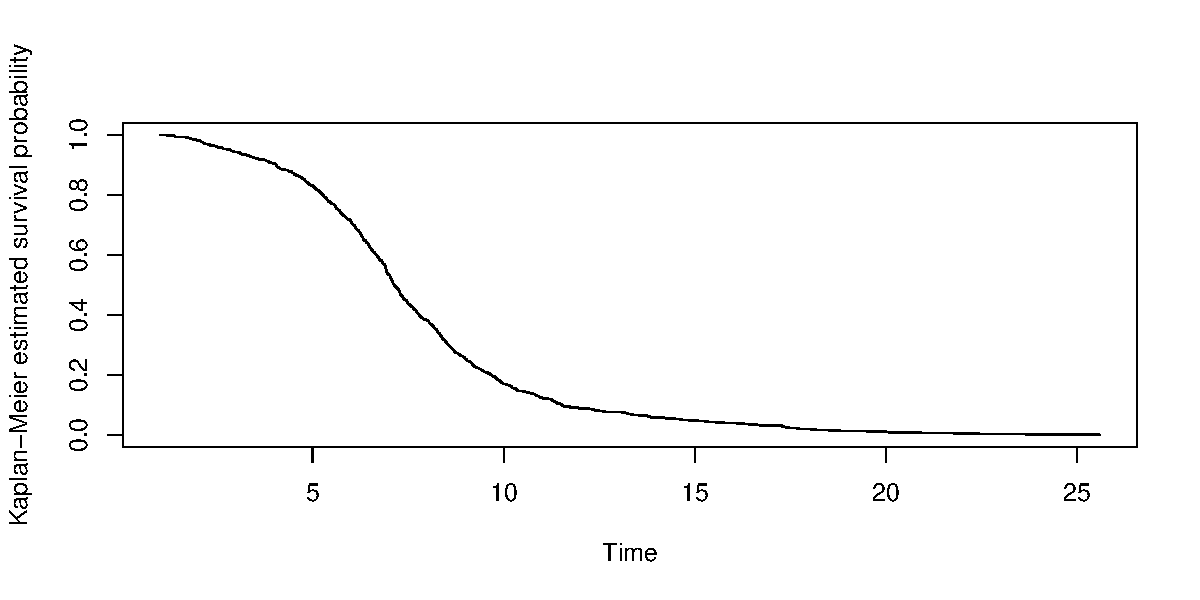
\includegraphics[scale=0.4]{figures/case1.pdf}
\end{figure}
Figure \ref{fig:boosting-ML-fixed-only} shows a plot of the negative log likelihood of the data (in-sample loss) as a function of iteration number.
The solid black line shows the boosting method as given above, where we estimate offsets $\beta_{1,0},\,\beta_{2,0}$ before we begin iterating.
These offsets are not changed.
We use numerical maximization to obtain the joint maximum likelihood estimates of our data set.
The offsets are $\hat{\beta}^{\text{ML}}_{1,0}=1.93$ and $\hat{\beta}^{\text{ML}}_{2,0}=0.18$.
Running the boosting algorithm to convergence, in this case 35 iterations, gives estimates of the offsets as $\hat{\beta}^{\text{ML}}_{1,0}=1.69$ and $\hat{\beta}^{\text{ML}}_{2,0}=0.16$, respectively.
We can see in the figure \ref{fig:boosting-ML-fixed-only} that it quite clearly does not reach the maximum likelihood value, which is the solid blue horizontal line.

Modifying the algorithm to incorporate (possibly) changing the intercept in each iteration did make the algorithm reach maximum likelihood.
To change the intercept in each iteration, we can perform a new numerical maximization after each boosting step.
This means to perform the same kind of numerical maximization as is done initially, before starting the iteration.
Only now using the estimated additive predictors as offsets.
With this setup, we decompose the additive predictor into steps.
We denote the initially estimated intercept $\beta_{1,0}$ as $\beta_{1,0}^{[0]}$.
The intercept in the additive predictor now becomes a sum of boosted intercepts,
\begin{equation}
    \beta_{1,0}=\beta_{1,0}^{[0]}+\sum_{m=1}^{\mstop}\beta_{1,0}^{[m]},
\end{equation}
where each $\beta_{1,0}^{[m]}$ is a boost in the intercept estimated in step $m$ of the boosting algorithm.
This means that in iteration step $m$, we wish to estimate a boost $\beta_{1,0}^{[m]}$.
If we choose to boost parameter $k$, we change the intercept of $\eta_k$.
If $k$ is 1, we update the intercept for that parameter,
\begin{equation}
    \hat{\beta}_{1,0}^{[m]}=\argmin_{c}R(\eta_1^{[m]}+c,\eta_2^{[m]}),
\end{equation}
and if $k$ is 2, we update that intercept,
\begin{equation}
    \hat{\beta}_{2,0}^{[m]}=\argmin_{c}R(\eta_2^{[m]},\eta_2^{[m]}+c).
\end{equation}
The modified algorithm using intercepts is shown in the previous subsection, \ref{algo:fhtboost-with-intercept}.

When using this algorithm with \textit{changing} intercepts, the algorithm was successful in recovering the maximum likelihood value and parameters.
See table \ref{table:ML} for the values, and figure \ref{fig:boosting-ML-fixed-only} for a plot.
\begin{table}\caption{Parameter values of a model which reaches ML}\label{table:ML}
\begin{tabular}{l|rrrrrr}
    & $\beta_{1,0}$ & $f_{1,1}$ & $f_{1,2}$ & $\beta_{2,0}$ & $f_{2,1}$ & $f_{2,2}$ \\
\hline
Maximum likelihood estimate     &    1.93 &    0.12 &    0.18 &    -0.94 &    -0.08 &     0.10 \\
Fixed intercept &    1.69 &    0.10 &    0.16 &    -0.71 &    -0.05 &     0.07 \\
Changing intercept    &    1.92 &    0.11 &    0.17 &    -0.93 &    -0.07 &     0.09
\end{tabular}\end{table}

\begin{figure}\label{fig:boosting-ML-fixed-only}
\caption{Boosting does not recover the maximum likelihood estimates}
\centering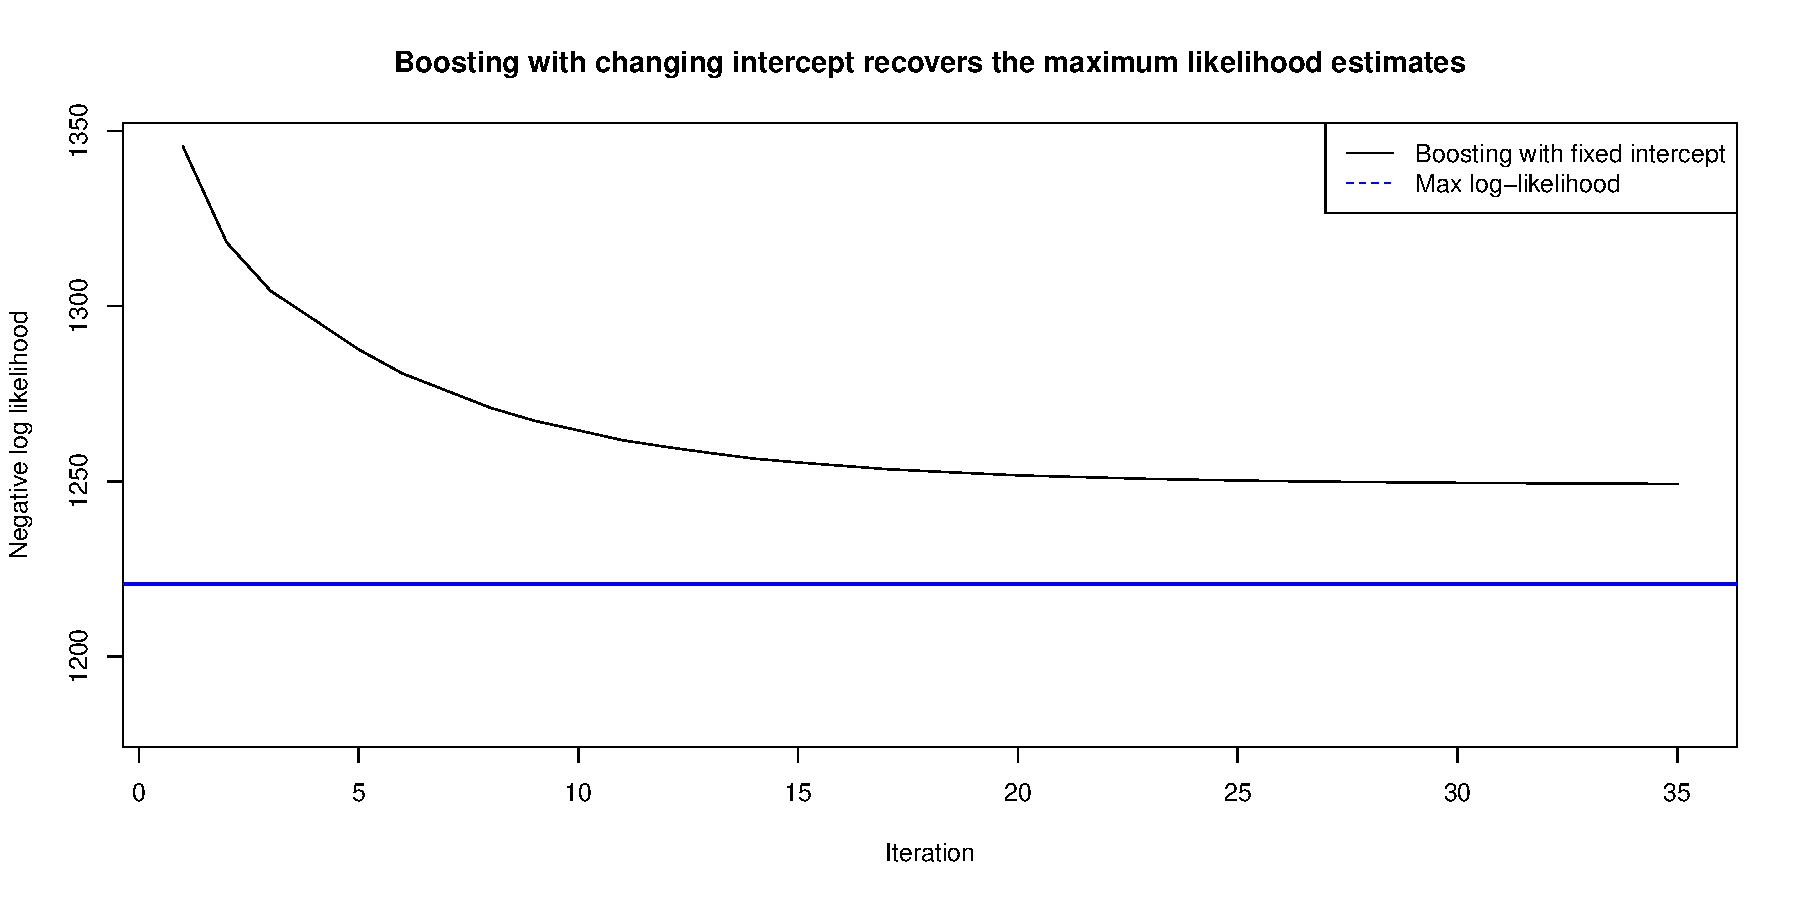
\includegraphics[scale=0.4]{figures/case1_fixed_only.pdf}
\end{figure}

\begin{figure}\label{fig:boosting-ML}
\caption{Boosting recovers the maximum likelihood estimates}
\centering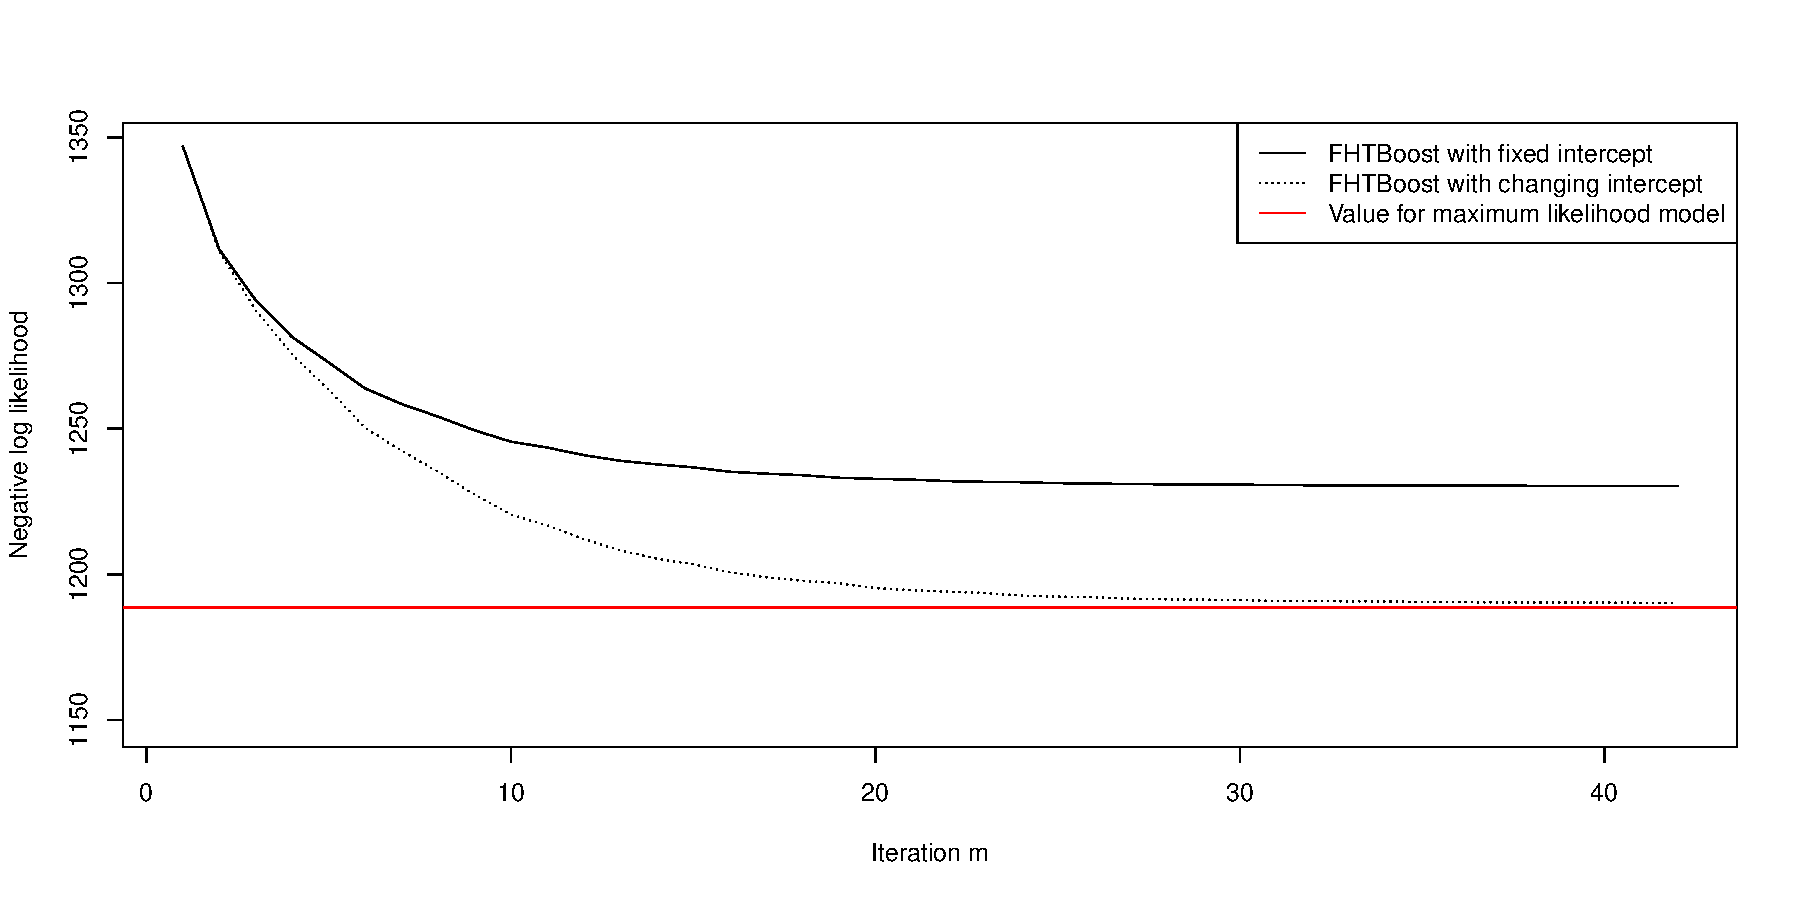
\includegraphics[scale=0.4]{figures/small_example.pdf}
\end{figure}